\section{Introduction}
To evaluate the modified methods, a dataset and a trained model where we can apply the methods is required.

The constituent Mauricio Reyes proposed the BraTS \cite{menze2015multimodal} dataset. This dataset contains
images of human brains taken with an MRI machine. The images are taken from patients which have brain tumors from the type
glioblastoma or lower grade glioma. The dataset contains four different types of images taken by the MRI machine (called modalities, the first four images in Figure \ref{brats_example}).

\begin{figure}[H]
\centering
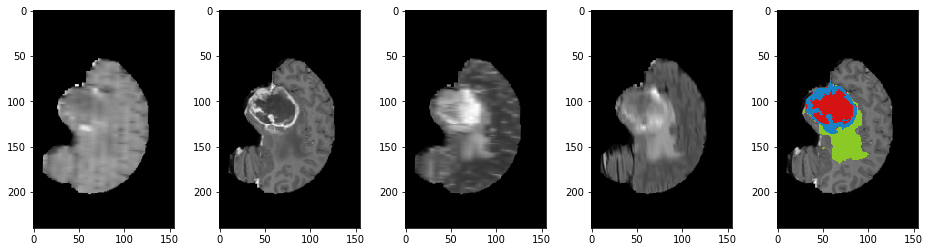
\includegraphics[width=14cm]{chapters/04_segmentation/images/brats.png}
\caption{One slice showing all 4 modalities and the tumor segmentation ground truth overlaid on the T1 contrast enhanced modality.}
\label{brats_example}
\end{figure}

In addition, the dataset contains ground truth labels. These labels mark the region in the brain where the tumor resides.
This segments further differentiate three different tissue types (see last image in Figure \ref{brats_example}).
These labels were manually drawn by physicians and validated by experienced neuro-radiologists.
The labels are saved in the same format as the scanner images, every type of tissue uses a specific integer value saved in the label file.
